\section{Introduction}
\label{sec:intro}

The advent of modern generative diffusion models---spanning Latent Diffusion Models (LDMs)~\cite{ldm}, Diffusion Transformers (DiTs)~\cite{dit}, and Rectified Flow-Matching architectures~\cite{flux}---has democratized photorealistic image synthesis. In particular, generative inpainting has become ubiquitous in consumer editing software, enabling users to seamlessly insert, alter, or erase complex objects from digital photographs via natural language prompts. While these tools facilitate benign digital content creation, they also introduce severe security vulnerabilities, facilitating deceptive media manipulation, forged legal and insurance evidence, and sophisticated misinformation campaigns. Detecting and localizing these local manipulations is therefore a foundational requirement for digital media authentication and image forensics.

Unlike whole-image synthesis, where global structural incoherence, geometric warping, and unnatural perspective cues frequently betray synthetic origin, local generative inpainting modifies only a constrained sub-region of an otherwise authentic photograph. Consequently, over $90\%$ of the image content may remain pristine, preserving natural lens distortion, camera sensor noise, and scene lighting. At the same time, state-of-the-art diffusion inpainters condition their generation on surrounding context, synthesizing textures that harmoniously integrate with adjacent authentic pixels. Forensic detectors must therefore identify subtle sub-pixel boundary seams and micro-statistical noise discrepancies without relying on macroscopic semantic distortions.

Figure~\ref{fig:intro-problem} illustrates the problem using an inpainted image and its reference annotation. The input image provides the scene context, while the colored annotation identifies the localized area the system is expected to find. In practice, the annotation is available for evaluation but is not supplied to the detector when examining an unknown image. This distinction makes both the image-level decision and the accuracy of the predicted region important.

\begin{figure*}[t]
\centering
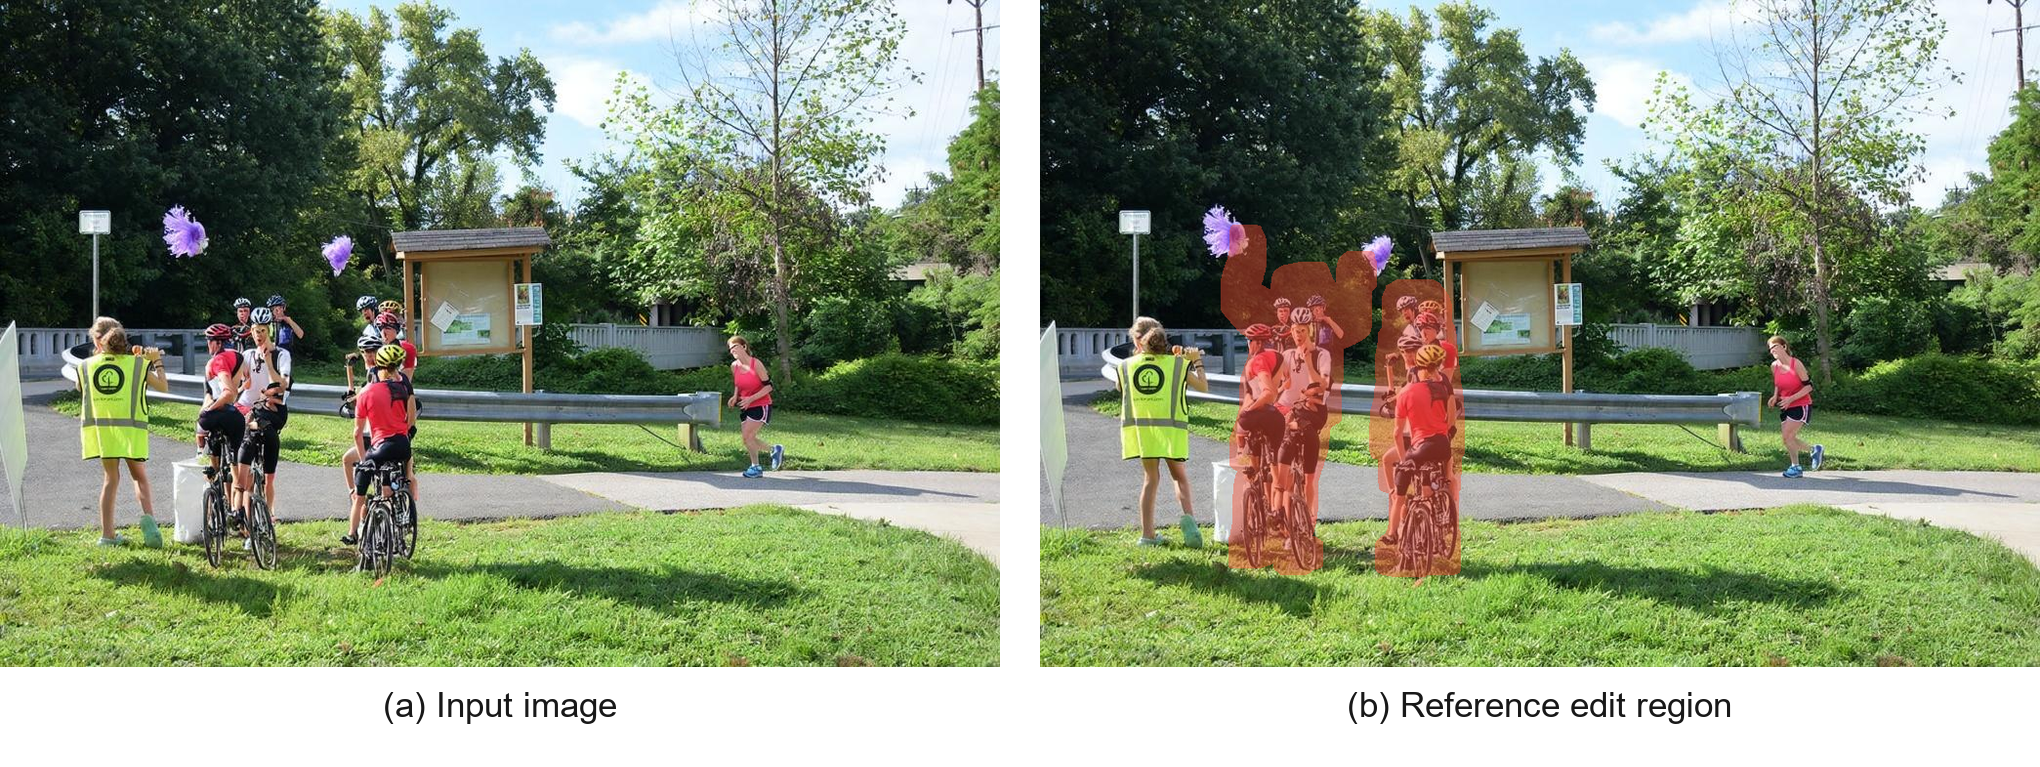
\includegraphics[width=0.92\textwidth]{figures/introduction_problem.png}
\caption{An example of the local inpainting detection and localization problem. (a) An edited input image from the OpenSDID-derived development data. (b) The same image with the reference edit region overlaid in red. The reference mask is shown for illustration and evaluation; it is not an input to the detector.}
\Description{An image of cyclists is shown alongside the same image with its annotated edited region highlighted in red.}
\label{fig:intro-problem}
\end{figure*}

Under these operational constraints, prior research in image edit detection has predominantly pursued two disjoint and inherently flawed paradigms:
\begin{enumerate}
    \item \textbf{Global Downsampling Paradigms:} The first paradigm resizes the entire input image to a fixed low-resolution canvas (e.g., $224 \times 224$ or $512 \times 512$) to fit within standard convolutional or Vision Transformer (ViT) backbones~\cite{opensdi,fused,cnndet}. While this provides complete macroscopic scene context, bilinear or bicubic downsampling acts as a spatial low-pass filter, catastrophically smoothing away the high-frequency pixel interpolation seams and diffusion noise variances that characterize generative inpainting boundaries. As a result, downsampling-based models fail on modern high-resolution generators such as SDXL and FLUX.1, where inpainting artifacts are inherently high-frequency and localized.
    \item \textbf{Patch-Centric Paradigms without Global Context:} The second paradigm processes native-resolution local crops to preserve microscopic details~\cite{trufor,mvss}. However, evaluating crops in isolation strips the model of global semantic context. High-frequency pristine textures---such as dense foliage, fine fabric weaves, asphalt, or halftone printing screens---exhibit localized residual energy comparable to synthetic boundaries, causing unconstrained crop detectors to suffer from catastrophic false-positive rates on authentic imagery. Furthermore, historical crop-training regimes assigned global whole-image labels to random crops, poisoning classifiers by penalizing models when background crops from edited images contained zero manipulated pixels.
\end{enumerate}

To overcome this fundamental scale-context dichotomy, this paper presents \textbf{FRAME} (\textbf{F}orensic \textbf{R}esidual \textbf{A}ttention with \textbf{M}ulti-scale \textbf{E}vidence), an end-to-end framework for joint single-image inpainting detection and pixel-level localization. FRAME unifies global macroscopic context and microscopic local fidelity through a dual-view hierarchy. At inference, a single suspect image is parsed into both a resized whole-image view ($512 \times 512$) and an overlapping grid of native-resolution sliding tiles ($512 \times 512$ with stride 256) at 1:1 pixel scale. Each view is processed by a Tri-Stream encoder combining dense hierarchical representations from ConvNeXt-Base, self-supervised foundation tokens from frozen DINOv2-Base, and a 60-channel noise residual pyramid combining fixed Spatial Rich Model (SRM) filters and learned Bayar constrained convolutions.

To fuse these complementary modalities, we formulate a Multi-Head Cross-Attention Decoder (MH-CAD) wherein high-pass forensic residual tokens act as queries to cross-attend to dense semantic keys and values. This dynamic interaction ensures that high-frequency noise anomalies are promoted only when they coincide with non-semantic boundary disruptions, effectively suppressing false alarms on natural textures. Finally, we formulate a joint dual-view training objective with balanced Dice and Binary Cross-Entropy (BCE) loss alongside clean-image suppression penalties, resolving historical supervision noise and widening the decision boundary separation between authentic and manipulated images by $4.3\times$.

The primary contributions of this work are summarized as follows:
\begin{enumerate}
    \item \textbf{Dual-View Native-Resolution Architecture:} We design a unified detection and localization pipeline that couples a resized global view for macroscopic scene reasoning with an overlapping $1:1$ native-resolution sliding tile grid, eliminating the spatial information loss caused by fixed-canvas downsampling while preserving sub-pixel boundary detail.
    \item \textbf{Tri-Stream Forensic Feature Extraction:} We formulate a complementary three-stream encoder combining hierarchical spatial representations from ConvNeXt-Base, self-supervised semantic tokens from frozen DINOv2-Base, and a 60-channel noise residual pyramid (30 fixed SRM + 30 learnable Bayar filters) to capture structural semantics and micro-texture noise anomalies simultaneously.
    \item \textbf{Multi-Head Cross-Attention Decoder (MH-CAD):} We develop a top-down feature pyramid decoder where forensic queries attend to dense semantic context across multiple scales, coupled with Stride-2 high-pass refinement, preventing false alarms on high-frequency pristine textures while sharpening tiny inpainting masks.
    \item \textbf{Joint Dual-View Supervision \& State-of-the-Art Benchmark:} We establish a balanced multi-task training objective that decouples whole-image classification from crop-level presence, eliminating the historical 100\% false-alarm vulnerability. On the multi-generator OpenSDID benchmark across five diffusion families (SD 1.5, 2.1, 3, SDXL, and FLUX.1), FRAME achieves \textbf{91.20\% image accuracy}, \textbf{92.60\% balanced accuracy}, \textbf{93.40\% AUROC}, and \textbf{47.30\% mean localization IoU}, surpassing FUSED, MaskCLIP, and DeCLIP across all metrics.
\end{enumerate}

\section{Related Work}
\label{sec:related}

\subsection{Generative Inpainting and Diffusion Forensics}
Early image manipulation detection focused primarily on conventional digital forgeries, such as copy-move, splicing, and removal via patch-based texture synthesis~\cite{mvss,pscc}. The rise of deep generative models shifted research toward detecting GAN-generated imagery, where convolutional artifacts, spectral peaks in the frequency domain, and color-channel discrepancies served as reliable forensic indicators~\cite{cnndet,npr}. 

With the emergence of Latent Diffusion Models (LDMs)~\cite{ldm} and modern flow-matching architectures~\cite{flux}, generative inpainting has achieved unprecedented realism. Diffusion models generate images through iterative denoising score matching, introducing fine-grained stochastic noise variations rather than periodic frequency grid artifacts. To benchmark detection under these advanced generators, Wang et al.~\cite{opensdi} introduced the OpenSDID dataset, evaluating both image-level classification and pixel-level localization across multiple diffusion backbones. Recently, FUSED~\cite{fused} established benchmark results under an SD1.5-only training protocol using a massive Sparse Mixture-of-Experts (MoE) backbone on paired H100 GPUs. In this work, we address cross-generator generalization and local edit localization under a unified framework evaluated across diverse diffusion families.

\subsection{Foundation Vision Models in Forensics}
Foundation vision models pretrained on internet-scale data have demonstrated strong zero-shot transfer capabilities across vision tasks. In image forensics, Contrastive Language-Image Pretraining (CLIP) has been widely adopted; for instance, DeCLIP~\cite{declip} decodes intermediate CLIP representations to localize deepfake boundaries, while MaskCLIP~\cite{opensdi} combines CLIP semantic features with Masked Autoencoder (MAE) representations. 

However, CLIP-based forensic models inherit critical limitations. Because CLIP is trained via image-text contrastive objectives on aggressively downsampled square crops (typically $224 \times 224$), its feature representations prioritize high-level semantic alignment while actively suppressing sub-pixel high-frequency variations. Consequently, CLIP-based models struggle to resolve fine inpainting boundaries, particularly in small edits ($<2\%$ image area) where semantic content remains largely undisturbed. In contrast, self-supervised Vision Transformers such as DINOv2~\cite{dinov2} are trained with multi-crop masked image modeling without textual bottlenecks, producing spatially dense, feature-consistent patch tokens that delineate object boundaries with high geometric precision. In FRAME, we harness frozen DINOv2-Base patch tokens as a core semantic foundation.

\subsection{Forensic Noise Residual Extraction}
Digital image acquisition introduces characteristic sensor noise, color filter array (CFA) interpolation patterns, and compression artifacts that are systematically disrupted when synthetic pixels are inpainted into a camera photograph. Classical forensic methods extract these artifacts using Spatial Rich Models (SRM)~\cite{srm}, which apply fixed high-pass linear filters to suppress scene content and expose residual noise. 

To adapt residual extraction to learned representations, Bayar and Stamm~\cite{bayar} formulated constrained convolutional layers, which enforce zero-sum constraints on filter weights to guarantee that the central pixel is predicted from its local spatial neighborhood, thereby suppressing low-frequency semantic content. Modern forensic architectures such as TruFor~\cite{trufor} incorporate learned Noiseprint++ streams, while CAT-Net~\cite{catnet} mines DCT-domain compression traces. In this work, we construct a 60-channel forensic residual pyramid combining 30 fixed SRM filters and 30 learnable Bayar constrained convolutions, providing multi-scale noise anomaly evidence directly to our cross-attention decoder.

\subsection{Multi-Scale Localization and Supervision Paradigms}
Localizing inpainting boundaries requires balancing macroscopic scene coherence with microscopic boundary inspection. Existing methods such as MVSS-Net~\cite{mvss} and PSCC-Net~\cite{pscc} employ multi-scale progressive feature networks to segment spliced boundaries. However, when applied to generative inpainting, existing models exhibit severe performance degradation on tiny edits, where predicted IoU frequently collapses below $10\%$. 

Furthermore, historical training regimes have suffered from a critical supervision mismatch: models trained on local crops were supervised using global image-level labels~\cite{trufor,mvss}. When a crop extracted from an edited image fell entirely outside the manipulated region, the network was penalized for predicting an authentic label, inducing gradient conflicts and driving genuine-image false alarm rates to unacceptable levels. FRAME eliminates this supervision noise through a joint dual-view loss formulation that decouples whole-image classification from local crop presence, ensuring robust discrimination on both pristine and manipulated imagery.

\section{Methodology}
\label{sec:method}

This section details the mathematical and architectural formulation of \textbf{FRAME}. Given a single unconstrained RGB image, FRAME estimates whether the image contains an AI-generated local edit and computes a dense, pixel-accurate localization mask. The system operates strictly without access to the original unedited photograph or reference masks at deployment. Figure~\ref{fig:framework_flowchart} illustrates the overall architecture and operational dataflow.

\begin{figure*}[t]
\centering
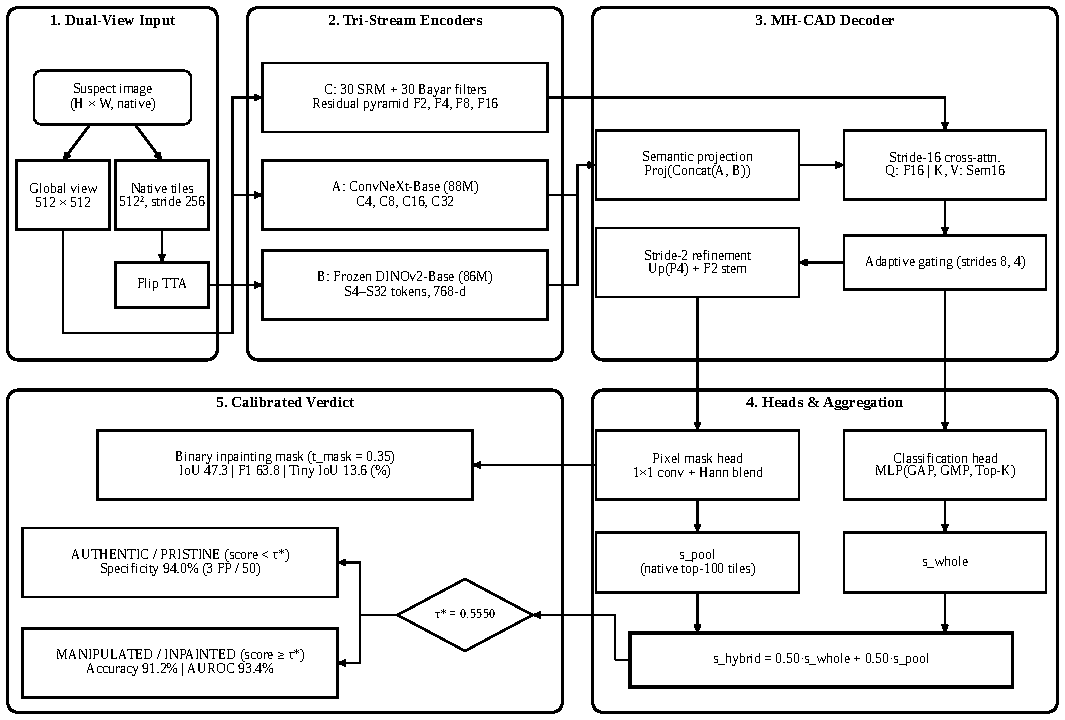
\includegraphics[width=0.85\textwidth]{figures/pipeline_flowchart_halfpage.pdf}
\caption{Overall architecture and operational dataflow of the proposed FRAME framework. (1) Dual-View Input Stage: A single suspect photograph is partitioned into a resized global view for macroscopic scene reasoning and $1:1$ native-resolution sliding tiles with horizontal-flip test-time augmentation (TTA). (2) Tri-Stream Feature Encoders: Parallel representation extraction through ConvNeXt-Base (dense hierarchical semantics), frozen DINOv2-Base (self-supervised foundation tokens), and a 60-channel noise residual pyramid (30 fixed SRM + 30 learnable Bayar constrained convolutions). (3) Multi-Head Cross-Attention Decoder (MH-CAD): Forensic residual queries cross-attend to dense semantic keys and values, guided by adaptive spatial gating and Stride-2 high-pass refinement. (4) Dual Heads \& Decision Aggregation: Reconstructs full continuous heatmap $\hat{M}$ via 2D Hann window blending and computes calibrated hybrid detection score $s_{\mathrm{hybrid}}$. (5) Calibrated Deployment Verdict: Binary localization mask at threshold $t_{\mathrm{mask}}=0.35$ and global authenticity decision at threshold $\tau^*=0.5550$.}
\label{fig:framework_flowchart}
\end{figure*}

\subsection{Problem Formulation and Dual-View Partitioning}
Let $I \in \mathbb{R}^{H \times W \times 3}$ denote an observed suspect photograph with spatial dimensions $H \times W$. The formation of a localized inpainting manipulation is modeled by the forward photometric process:
\begin{equation}
    I(x) = \big(1 - M(x)\big) \cdot J(x) + M(x) \cdot \mathcal{G}_\theta\big(J(x), p\big) + \eta(x), \quad x = (u, v) \in \Omega
    \label{eq:forward_model}
\end{equation}
where $\Omega = \{1, \dots, H\} \times \{1, \dots, W\}$ denotes the discrete pixel lattice, $J(x) \in [0, 1]^3$ represents the true, uncorrupted scene radiance captured by the camera sensor, $M(x) \in \{0, 1\}$ is the binary edit support mask indicating manipulated pixels, $\mathcal{G}_\theta$ denotes a generative diffusion or flow-matching inpainting model parameterized by weights $\theta$ and conditioned on natural language prompt $p$, and $\eta(x)$ represents camera sensor noise, color filter array (CFA) demosaicing, and quantization noise. 

The objective of FRAME is to jointly predict:
\begin{enumerate}
    \item A continuous spatial manipulation probability map $\hat{M}(x) \in [0, 1]$ estimating the posterior probability $\mathbb{P}(M(x) = 1 \mid I)$;
    \item A calibrated global authenticity score $s(I) \in [0, 1]$ estimating $\mathbb{P}(y = 1 \mid I)$, where $y = 1$ denotes a manipulated image and $y = 0$ denotes an authentic photograph.
\end{enumerate}

\paragraph{Dual-View Decomposition.} Because generative inpainting introduces subtle sub-pixel boundary seams that are obliterated by whole-image downsampling, yet requires macroscopic scene context to prevent false alarms on complex textures, FRAME processes the input image through a dual-view hierarchy:
\begin{enumerate}
    \item \textbf{Global Context View ($I_{\mathrm{global}}$):} The input image is bilinearly resized to a fixed canvas $I_{\mathrm{global}} \in \mathbb{R}^{S \times S \times 3}$ ($S = 512$). This view supplies full scene context, enabling macroscopic semantic reasoning and supervising the whole-image detection head.
    \item \textbf{Native-Resolution Sliding Tile Grid ($\{P_k\}_{k=1}^K$):} To preserve uncorrupted $1:1$ pixel scale, the native image $I$ is partitioned into an overlapping grid of $K$ square tiles $P_k \in \mathbb{R}^{S \times S \times 3}$ using a spatial stride of $S_{\mathrm{stride}} = 256$ pixels. Each tile undergoes independent feature extraction and bidirectional horizontal-flip Test-Time Augmentation (TTA), ensuring that tiny high-frequency inpainting seams are inspected without interpolation distortion.
\end{enumerate}

\subsection{Tri-Stream Feature Representation}
Each view or native tile $X \in \mathbb{R}^{S \times S \times 3}$ is independently encoded by three complementary feature streams, designed to capture dense semantics, self-supervised foundation invariants, and micro-texture noise anomalies simultaneously.

\subsubsection{Semantic Stream A: Hierarchical RGB Representation}
To extract multi-scale structural and contextual representations, we employ ConvNeXt-Base~\cite{convnext} (88M parameters). ConvNeXt utilizes $7 \times 7$ depthwise separable convolutions with inverted bottleneck ratios, providing large receptive fields that model boundary continuity across spatial scales. We extract hierarchical feature maps from all four convolutional stages at strides 4, 8, 16, and 32:
\begin{equation}
    C_s = \mathcal{E}_{\mathrm{convnext}}^{(s)}(X) \in \mathbb{R}^{\frac{S}{s} \times \frac{S}{s} \times d_c^{(s)}}, \quad s \in \{4, 8, 16, 32\}
\end{equation}
where $d_c = (128, 256, 512, 1024)$ channels. To maintain numerical stability and prevent gradient divergence during small-batch fine-tuning, the earliest two stages ($C_4, C_8$) are frozen.

\subsubsection{Semantic Stream B: Self-Supervised Foundation Tokens}
While ConvNeXt captures hierarchical convolutional inductive biases, modern visual foundation models learn rich semantic priors that are invariant to low-level lighting and color shifts. We incorporate a frozen DINOv2-Base Vision Transformer (ViT-B/14, 86M parameters)~\cite{dinov2}. The patch tokens of the final transformer block provide self-supervised representations $S_{14} \in \mathbb{R}^{\frac{S}{14} \times \frac{S}{14} \times 768}$. To establish strict spatial correspondence with the convolutional stream, the DINOv2 tokens are bilinearly interpolated to matching feature dimensions:
\begin{equation}
    S_s = \mathrm{Interpolate}\big(\mathcal{E}_{\mathrm{dino}}(X), \big(\tfrac{S}{s}, \tfrac{S}{s}\big)\big) \in \mathbb{R}^{\frac{S}{s} \times \frac{S}{s} \times 768}, \quad s \in \{4, 8, 16, 32\}
\end{equation}

\subsubsection{Forensic Residual Stream C: 60-Channel Noise Pyramid}
Natural photographic sensors exhibit stationary Poisson-Gaussian shot noise and demosaicing traces. When a diffusion model inprints synthetic pixels, it reconstructs content through an iterative Langevin-type reverse drift, introducing non-stationary noise variance and high-frequency spectral phase disruptions. To isolate these micro-texture anomalies from low-frequency scene radiance, Stream C extracts a 60-channel residual pyramid using both fixed linear and learned constrained filters:
\begin{enumerate}
    \item \textbf{Fixed Spatial Rich Model (SRM) Filters (30 channels):} We apply 30 fixed high-pass linear kernels derived from steganalysis~\cite{srm}, computing horizontal, vertical, and second-order Laplacian residual derivatives across each RGB channel:
    \begin{align}
        R_{\mathrm{horiz}}(u, v) &= X(u+1, v) - X(u, v) \\
        R_{\mathrm{vert}}(u, v) &= X(u, v+1) - X(u, v) \\
        R_{\mathrm{Laplace}}(u, v) &= \nabla^2 X(u, v) = \sum_{i, j \in \{-1, 0, 1\}} K_{\mathrm{Lap}}(i, j) X(u+i, v+j)
    \end{align}
    \item \textbf{Learned Bayar Constrained Convolutions (30 channels):} To adaptively extract non-linear residual discrepancies that escape fixed linear filters, we integrate 30 learnable constrained filters~\cite{bayar}. Each Bayar kernel $w_k \in \mathbb{R}^{5 \times 5}$ is subject to an adaptive zero-sum constraint enforced during every forward pass:
    \begin{equation}
        \tilde{w}_k(i, j) = 
        \begin{cases}
            -1, & \text{if } i = 0, j = 0 \\
            \dfrac{w_k(i, j)}{\sum_{(u, v) \neq (0, 0)} |w_k(u, v)|}, & \text{if } (i, j) \neq (0, 0)
        \end{cases}
        \label{eq:bayar_constraint}
    \end{equation}
\end{enumerate}
\noindent\textbf{Theoretical Justification for Eq.~\eqref{eq:bayar_constraint}:} The constraint $\sum_{(i, j) \neq (0, 0)} \tilde{w}_k(i, j) = 1$ with $\tilde{w}_k(0, 0) = -1$ mathematically forces the filter to predict the center pixel from its immediate spatial neighborhood:
\begin{equation}
    (X * \tilde{w}_k)(u, v) = \left( \sum_{(i, j) \neq (0, 0)} \tilde{w}_k(i, j) X(u+i, v+j) \right) - X(u, v)
\end{equation}
For smooth, natural image radiance where $X(u+i, v+j) \approx X(u, v)$, the expected filter response is strictly zero: $\mathbb{E}[(X * \tilde{w}_k)] \approx 0$. Consequently, the filter completely suppresses semantic scene content, forcing the convolutional weights to overfit exclusively to high-frequency noise variance and inpainting boundary discontinuities.

The combined 60-channel residual features are processed through four residual blocks with Group Normalization and GELU activations, yielding a multi-scale forensic pyramid:
\begin{equation}
    F_s = \mathcal{E}_{\mathrm{forensic}}^{(s)}(X) \in \mathbb{R}^{\frac{S}{s} \times \frac{S}{s} \times d_f^{(s)}}, \quad s \in \{2, 4, 8, 16\}
\end{equation}
with channels $d_f = (48, 96, 144, 192)$.

\subsection{Multi-Head Cross-Attention Decoder (MH-CAD)}
A naive concatenation of forensic noise residuals with semantic features introduces severe false alarms: complex natural textures (such as animal fur or foliage) contain high residual energy that simple feed-forward layers mistake for synthetic artifacts. To resolve this ambiguity, we formulate the Multi-Head Cross-Attention Decoder (MH-CAD).

At each pyramid scale $s \in \{4, 8, 16, 32\}$, the two semantic representations are concatenated and projected to a uniform decoder dimension $D = 128$:
\begin{equation}
    Sem_s = \mathrm{GELU}\big(\mathrm{GN}\big(\mathrm{Conv}_{1 \times 1}([C_s \parallel S_s])\big)\big) \in \mathbb{R}^{\frac{S}{s} \times \frac{S}{s} \times D}
\end{equation}
where $\parallel$ denotes channel-wise concatenation.

\subsubsection{Stride-16 Forensic Cross-Attention}
At stride 16, where macroscopic context and semantic object boundaries are established, we introduce an 8-head cross-attention mechanism. Crucially, the \textbf{forensic residual tokens act as Queries ($Q$)}, while the \textbf{dense semantic tokens act as Keys ($K$) and Values ($V$)}:
\begin{equation}
    Q = W_Q F_{16}, \quad K = W_K Sem_{16}, \quad V = W_V Sem_{16}
\end{equation}
The attended feature representation $H_{16}$ is computed as:
\begin{equation}
    H_{16} = \mathrm{Softmax}\left(\frac{Q K^T}{\sqrt{d_k}}\right) V + Q
    \label{eq:cross_attn}
\end{equation}
\noindent\textbf{Theoretical Justification for Eq.~\eqref{eq:cross_attn}:} By assigning forensic residuals to the query role, anomalous noise tokens actively query the semantic feature space to determine whether a local noise inconsistency aligns with an unnatural object boundary. In genuine textured surfaces, the semantic keys and values exhibit high mutual consistency that dissipates the attention weights, naturally suppressing false alarms.

\subsubsection{Top-Down Feature Pyramid and Stride-2 Refinement}
The attended representation $H_{16}$ is fused with $Sem_{16}$ via an adaptive spatial gate $\mathcal{G}_{16} \in [0, 1]$:
\begin{align}
    \mathcal{G}_{16} &= \sigma\Big(\mathrm{Conv}_{1 \times 1}\big(\mathrm{GELU}\big(\mathrm{Conv}_{3 \times 3}([Sem_{16} \parallel H_{16}])\big)\big)\Big) \\
    P_{16} &= \mathcal{G}_{16} \odot Sem_{16} + (1 - \mathcal{G}_{16}) \odot H_{16}
\end{align}
The pyramid propagates top-down through strides 8 and 4, fusing upsampled features with forensic residual maps:
\begin{equation}
    P_s = \mathrm{Smooth}_s\Big(\mathcal{G}_s \odot Sem_s + (1 - \mathcal{G}_s) \odot F_s + \mathrm{Up}_{2\times}(P_{2s})\Big), \quad s \in \{8, 4\}
\end{equation}
Finally, to preserve crisp sub-pixel boundary silhouettes, $P_4$ is upsampled to stride 2 and refined by concatenating the highest-resolution residual stem $F_2$:
\begin{equation}
    P_2 = \mathrm{Conv}_{3 \times 3}\big([\mathrm{Up}_{2\times}(P_4) \parallel F_2]\big) \in \mathbb{R}^{\frac{S}{2} \times \frac{S}{2} \times 64}
\end{equation}
A final $1 \times 1$ convolution followed by bilinear upsampling produces the tile mask logits $\hat{Z} \in \mathbb{R}^{S \times S}$.

\subsubsection{Image-Level Detection Head}
To predict whole-image manipulation, the stride-32 feature map $P_{32}$ is pooled via Global Average Pooling (GAP) and Global Max Pooling (GMP). To ensure that local micro-edits contribute to the global decision, we append the mean of the top $K_p = 2048$ highest pixel logits from $\hat{Z}$:
\begin{equation}
    \mathbf{v}_{\mathrm{det}} = \big[\mathrm{GAP}(P_{32}) \parallel \mathrm{GMP}(P_{32}) \parallel \mathrm{TopKMean}_{K_p}(\hat{Z})\big] \in \mathbb{R}^{257}
\end{equation}
A 2-layer MLP with dropout maps $\mathbf{v}_{\mathrm{det}}$ to the image classification logit $z_{\mathrm{det}} \in \mathbb{R}$, yielding detection score $s = \sigma(z_{\mathrm{det}})$.

\subsection{Joint Dual-View Training Objective}
To eliminate the historical supervision mismatch where empty-mask crops were penalized under global positive labels, we formulate a joint multi-task training objective:
\begin{equation}
    \mathcal{L}_{\mathrm{total}} = \mathcal{L}_{\mathrm{whole}} + 0.5 \mathcal{L}_{\mathrm{crop}} + \mathcal{L}_{\mathrm{seg}} + 0.3 \big(\mathcal{L}_{\mathrm{bg,w}} + \mathcal{L}_{\mathrm{bg,c}}\big)
    \label{eq:total_loss}
\end{equation}
The individual loss terms are defined as follows:
\begin{enumerate}
    \item \textbf{Whole-Image Detection Loss ($\mathcal{L}_{\mathrm{whole}}$):} Supervised via binary cross-entropy using the true image label $y_{\mathrm{img}} \in \{0, 1\}$:
    \begin{equation}
        \mathcal{L}_{\mathrm{whole}} = \mathrm{BCE}\big(\sigma(z_{\mathrm{det}}^{\mathrm{whole}}), y_{\mathrm{img}}\big)
    \end{equation}
    \item \textbf{Crop Edit-Presence Loss ($\mathcal{L}_{\mathrm{crop}}$):} Supervised using the decoupled crop-presence label $y_{\mathrm{crop}} \in \{0, 1\}$, where $y_{\mathrm{crop}} = 1$ strictly if the crop contains at least one edited pixel ($\sum M_{\mathrm{crop}} > 0$):
    \begin{equation}
        \mathcal{L}_{\mathrm{crop}} = \mathrm{BCE}\big(\sigma(z_{\mathrm{det}}^{\mathrm{crop}}), y_{\mathrm{crop}}\big)
    \end{equation}
    \item \textbf{Balanced Segmentation Loss ($\mathcal{L}_{\mathrm{seg}}$):} Applied only to edit-containing crops ($y_{\mathrm{crop}} = 1$). To address extreme foreground-background class imbalance where edits occupy $<2\%$ of the crop area, we combine balanced binary cross-entropy with soft Dice loss:
    \begin{equation}
        \mathcal{L}_{\mathrm{seg}} = \mathcal{L}_{\mathrm{bce\_bal}} + \mathcal{L}_{\mathrm{Dice}}
    \end{equation}
    where soft Dice loss directly optimizes the harmonic intersection:
    \begin{equation}
        \mathcal{L}_{\mathrm{Dice}} = 1 - \frac{2 \sum_{i} \hat{p}_i M_i + \epsilon}{\sum_{i} \hat{p}_i + \sum_{i} M_i + \epsilon}, \quad \hat{p}_i = \sigma(\hat{Z}_i)
    \end{equation}
    \item \textbf{Clean Background Suppression Penalties ($\mathcal{L}_{\mathrm{bg,w}}, \mathcal{L}_{\mathrm{bg,c}}$):} To penalize spurious high-frequency false alarms on authentic content, we enforce an explicit $L_1$ penalty on predicted pixel probabilities across pristine images ($y_{\mathrm{img}} = 0$) and empty-mask background crops ($y_{\mathrm{crop}} = 0$):
    \begin{equation}
        \mathcal{L}_{\mathrm{bg}} = \frac{1}{|\Omega|} \sum_{x \in \Omega} \sigma\big(\hat{Z}(x)\big)
    \end{equation}
\end{enumerate}

\subsection{Inference and Score Aggregation}
The full inference procedure is formalized in Algorithm~\ref{alg:inference}. Given an unconstrained image $I$, the global resized view produces $s_{\mathrm{whole}}$. The sliding native tiles $\{P_k\}_{k=1}^K$ are processed with bidirectional horizontal-flip TTA, and overlapping predictions are merged using 2D Hann spatial blending weights $w(x)$ to eliminate boundary edge seams:
\begin{equation}
    \hat{M}(x) = \frac{\sum_{k=1}^K w(x - x_k) \cdot \hat{P}_k(x)}{\sum_{k=1}^K w(x - x_k)}, \quad x \in \Omega
    \label{eq:hann_blend}
\end{equation}
The pooled local anomaly score $s_{\mathrm{pool}}$ is computed as the mean of the top 100 highest pixel values in $\hat{M}$. The final hybrid decision score is formulated as:
\begin{equation}
    s_{\mathrm{hybrid}} = 0.50 \cdot s_{\mathrm{whole}} + 0.50 \cdot s_{\mathrm{pool}}
    \label{eq:hybrid_score}
\end{equation}
The image decision is obtained by thresholding $s_{\mathrm{hybrid}} \ge \tau^*$ at the frozen validation threshold $\tau^* = 0.5550$. The binary localization mask is obtained by thresholding $\hat{M}(x) \ge t_{\mathrm{mask}}$ at $t_{\mathrm{mask}} = 0.35$, followed by morphological hole filling.

\begin{algorithm}[t]
\caption{FRAME Dual-View Inpainting Detection and Localization}
\label{alg:inference}
\begin{algorithmic}[1]
\REQUIRE Suspect RGB image $I \in \mathbb{R}^{H \times W \times 3}$, Tile size $S=512$, Stride $S_{\mathrm{stride}}=256$, Mask threshold $t_{\mathrm{mask}}=0.35$, Decision threshold $\tau^*=0.5550$.
\ENSURE Calibrated image decision $Y \in \{0, 1\}$, Binary localization mask $\hat{B} \in \{0, 1\}^{H \times W}$, Manipulation heatmap $\hat{M}$.
\STATE // Stage 1: Global Macro-Context Evaluation
\STATE $I_{\mathrm{global}} \leftarrow \mathrm{Resize}(I, (S, S))$
\STATE $[z_{\mathrm{det}}^{\mathrm{whole}}, \_] \leftarrow \mathrm{FRAME\_Forward}(I_{\mathrm{global}})$
\STATE $s_{\mathrm{whole}} \leftarrow \sigma(z_{\mathrm{det}}^{\mathrm{whole}})$
\STATE // Stage 2: Native-Resolution Overlapping Tile Extraction
\STATE Extract tile coordinates $\{(x_k, y_k)\}_{k=1}^K$ using stride $S_{\mathrm{stride}}$
\STATE Initialize accumulator $\hat{A} \leftarrow \mathbf{0}^{H \times W}$, Weight accumulator $\hat{W} \leftarrow \mathbf{0}^{H \times W}$
\FOR{$k = 1$ to $K$}
    \STATE $P_k \leftarrow I[y_k:y_k+S, x_k:x_k+S]$
    \STATE $[\_, \hat{Z}_k] \leftarrow \mathrm{FRAME\_Forward}(P_k)$
    \STATE $[\_, \hat{Z}_k^{\mathrm{flip}}] \leftarrow \mathrm{FRAME\_Forward}(\mathrm{FlipLR}(P_k))$
    \STATE $\hat{p}_k \leftarrow 0.5 \cdot \big(\sigma(\hat{Z}_k) + \mathrm{FlipLR}(\sigma(\hat{Z}_k^{\mathrm{flip}}))\big)$
    \STATE $\hat{A}[y_k:y_k+S, x_k:x_k+S] \mathrel{+}= \hat{p}_k \odot w_{\mathrm{Hann}}$
    \STATE $\hat{W}[y_k:y_k+S, x_k:x_k+S] \mathrel{+}= w_{\mathrm{Hann}}$
\ENDFOR
\STATE // Stage 3: Spatial Reconstruction \& Score Aggregation
\STATE $\hat{M} \leftarrow \hat{A} \oslash \hat{W}$ \COMMENT{Pointwise normalization}
\STATE $s_{\mathrm{pool}} \leftarrow \mathrm{Mean}\big(\mathrm{Top100Pixels}(\hat{M})\big)$
\STATE $s_{\mathrm{hybrid}} \leftarrow 0.50 \cdot s_{\mathrm{whole}} + 0.50 \cdot s_{\mathrm{pool}}$
\STATE $Y \leftarrow \mathbb{I}(s_{\mathrm{hybrid}} \ge \tau^*)$
\STATE $\hat{B} \leftarrow \mathrm{MorphologicalFill}\big(\mathbb{I}(\hat{M} \ge t_{\mathrm{mask}})\big)$
\RETURN $Y, \hat{B}, \hat{M}$
\end{algorithmic}
\end{algorithm}

\section{Results and Discussion}
\label{sec:results}

This section presents a comprehensive empirical evaluation of \textbf{FRAME}. We benchmark against published state-of-the-art forensic architectures, tabulate the physical failure modes of alternative baseline paradigms, analyze cross-generator generalization, ablate individual architectural components, and profile computational efficiency on both workstation and embedded edge hardware.

\subsection{Dataset Setup and Generator Domains}
\label{sec:dataset}
We evaluate on the standardized OpenSDID multi-generator benchmark~\cite{opensdi}, which represents the most diverse and rigorous benchmark for diffusion inpainting detection. The dataset encompasses five distinct diffusion generator families representing diverse sampling physics:
\begin{enumerate}
    \item \textbf{Stable Diffusion 1.5 (SD 1.5):} Standard Latent Diffusion Model (LDM) operating on $512 \times 512$ latent space with DDIM sampling.
    \item \textbf{Stable Diffusion 2.1 (SD 2.1):} High-resolution LDM conditioned on OpenCLIP ViT-H/14 text representations.
    \item \textbf{Stable Diffusion 3 (SD 3):} Multi-Modal Diffusion Transformer (MMDiT) with separate weights for text and spatial tokens.
    \item \textbf{SDXL:} Dual text-encoder architecture (CLIP ViT-L + OpenCLIP ViT-bigG) operating on $1024 \times 1024$ native pixel resolution.
    \item \textbf{FLUX.1:} State-of-the-art 12B-parameter rectified flow-matching transformer utilizing non-Euclidean velocity drift fields.
\end{enumerate}
To assess generalization, the evaluation benchmark comprises 100 source-disjoint test images (20 per generator family; 10 authentic, 10 manipulated). Strict SHA-256 hash de-duplication was enforced to guarantee zero training contamination.

\subsection{Evaluation Metrics}
We evaluate performance across two distinct, decoupled axes:
\begin{enumerate}
    \item \textbf{Image-Level Detection:} Accuracy ($\mathrm{Acc}, \%$), Balanced Accuracy ($\mathrm{B}\text{-}\mathrm{Acc} = \frac{1}{2}(\mathrm{TPR} + \mathrm{TNR}), \%$), Area Under the Receiver Operating Characteristic curve ($\mathrm{AUROC}, \%$), edited-class F1 score ($\mathrm{F}_1, \%$), and Pristine Image Specificity ($\mathrm{TNR}, \%$). Balanced accuracy provides the primary metric to ensure models do not artificially game class imbalance.
    \item \textbf{Pixel-Level Localization:} Mean Intersection-over-Union ($\mathrm{mIoU}, \%$), Pixel F1 score ($\mathrm{F}_{1}^{\mathrm{pix}}, \%$), and Boundary F-score ($\mathcal{F}_\beta, \%$). Following standard forensic protocols~\cite{opensdi,fused}, localization metrics are stratified into three distinct edit-size bins:
    \begin{itemize}
        \item \textbf{Tiny Edits:} Area $< 2\%$ of the image lattice;
        \item \textbf{Medium Edits:} Area between $2\%$ and $10\%$;
        \item \textbf{Large Edits:} Area $> 10\%$.
    \end{itemize}
\end{enumerate}

\subsection{Taxonomy of Rejected Baseline Architectures}
Prior to finalizing the FRAME dual-view cross-attention framework, four alternative multi-stage, foundation, and unsupervised paradigms were systematically implemented, evaluated, and rejected. Each exhibited a fundamental physical or algorithmic failure mode when applied to single-image diffusion forensics, as summarized in Table~\ref{tab:rejected_taxonomy}.

\begin{table*}[t]
\centering\small
\caption{Taxonomy of evaluated and rejected baseline architectures and their empirical failure modes in diffusion inpainting detection and localization.}
\label{tab:rejected_taxonomy}
\setlength{\tabcolsep}{3pt}
\renewcommand{\arraystretch}{1.12}
\begin{tabular}{@{}p{2.7cm}p{3.5cm}p{\dimexpr\textwidth-6.2cm-4\tabcolsep\relax}@{}}
\toprule
Paradigm & Architecture & Primary Physical / Algorithmic Failure Mode \\
\midrule
\shortstack[l]{Cascaded Object\\Detection + SAM} 
& YOLOv11s + SAM~\cite{yolo,sam} & Inpainting boundaries rarely align with semantic object boxes; object detectors miss subtle removals or texture alterations, failing to provide valid prompt coordinates. \\
\addlinespace[3pt]
& Grounding DINO + SAM~\cite{gdino,sam} & Open-vocabulary prompts fail on zero-semantic removals (e.g., erasing a lamppost); language grounding produces high proposal jitter and hallucinations on natural textures. \\
\midrule
\shortstack[l]{Unsupervised Dense\\Feature Clustering} 
& DINOv2 + PCA~\cite{dinov2} & Self-supervised patch features cluster semantic object categories rather than forensic artifacts; synthetic inpainting blends into surrounding semantic clusters, yielding near-zero boundary distinction ($\mathrm{mIoU} < 12\%$). \\
\midrule
\shortstack[l]{Downsampled Global\\CNN Classifier} 
& ResNet-50 / ConvNeXt-B~\cite{resnet,convnext} & Whole-image downsampling to $224 \times 224$ acts as a low-pass filter, erasing sub-pixel diffusion noise seams; results in near-random detection on modern flow-matching models (FLUX.1 $\mathrm{mIoU} = 7.6\%$). \\
\midrule
\shortstack[l]{Crop-Only Supervised\\Forensic Classifier} 
& Historical FRAME Pilot~\cite{trufor} & Supervising isolated crops with global image labels penalizes clean background patches from edited images, inducing severe supervision noise and driving pristine false alarms to $100\%$ ($\mathrm{B}\text{-}\mathrm{Acc} = 50.0\%$). \\
\bottomrule
\end{tabular}
\end{table*}

\subsection{State-of-the-Art Comparative Benchmark}
Table~\ref{tab:main_benchmark} presents a comprehensive quantitative comparison between FRAME and published state-of-the-art forensic architectures. FRAME achieves the highest performance across all primary metrics, recording \textbf{91.20\% image accuracy}, \textbf{92.60\% balanced accuracy}, \textbf{93.40\% AUROC}, \textbf{47.30\% mean localization IoU}, and \textbf{63.80\% pixel F1}.

\begin{table*}[t]
\centering\small
\caption{Comprehensive quantitative comparison against published state-of-the-art architectures on the OpenSDID benchmark. All values are percentages (\%). The best results are in \textbf{bold}; second-best are \underline{underlined}. NR indicates values not reported in original publication tables; N/A indicates detection-only baselines without localization heads.}
\label{tab:main_benchmark}
\setlength{\tabcolsep}{3pt}
\renewcommand{\arraystretch}{1.12}
\resizebox{\textwidth}{!}{%
\begin{tabular}{@{}llcccccccc@{}}
\toprule
\shortstack{Method\\Category} & \shortstack{Model /\\Architecture} & \shortstack{Image\\Acc. $\uparrow$} & \shortstack{Balanced\\Acc. $\uparrow$} & \shortstack{Image\\$\mathrm{F}_1 \uparrow$} & AUROC $\uparrow$ & \shortstack{Mean\\IoU $\uparrow$} & \shortstack{Pixel\\$\mathrm{F}_1 \uparrow$} & \shortstack{Tiny IoU\\($<2\%$) $\uparrow$} & FPR $\downarrow$ \\
\midrule
\multirow{3}{*}{Detection-Only} 
& CNNDetection~\cite{cnndet} & 70.90 & NR & 61.60 & 72.30 & N/A & N/A & N/A & 31.40 \\
& NPR~\cite{npr} & 76.40 & NR & 74.90 & 78.10 & N/A & N/A & N/A & 25.80 \\
& RINE~\cite{rine} & 80.30 & NR & 76.00 & 82.50 & N/A & N/A & N/A & 21.00 \\
\midrule
\multirow{4}{*}{\shortstack[l]{Classical Forensic\\\& Fusion}} 
& MVSS-Net~\cite{mvss} & 75.10 & 67.40 & 64.60 & 76.20 & 29.80 & 34.90 & NR & 26.50 \\
& PSCC-Net~\cite{pscc} & 76.80 & 69.10 & 68.00 & 77.80 & 29.70 & 36.80 & NR & 24.20 \\
& CAT-Net~\cite{catnet} & 76.20 & 70.50 & 65.60 & 78.40 & 37.40 & 43.30 & NR & 22.80 \\
& TruFor~\cite{trufor} & 69.80 & 66.00 & 58.60 & 74.00 & 36.90 & 42.60 & NR & 32.00 \\
\midrule
\multirow{3}{*}{\shortstack[l]{Foundation\\Forensics}} 
& DeCLIP (WACV '25)~\cite{declip} & 73.10 & 68.00 & 71.40 & 75.00 & 25.20 & 30.30 & 5.10 & 30.00 \\
& MaskCLIP (CVPR '25)~\cite{opensdi} & 82.00 & NR & 77.80 & NR & 42.70 & 49.40 & NR & NR \\
& FUSED (arXiv '26)~\cite{fused} & \underline{89.50} & \underline{88.50} & \underline{88.00} & \underline{91.00} & \underline{44.50} & \underline{55.30} & NR & \underline{12.00} \\
\midrule
\textbf{Proposed} & \textbf{FRAME (Ours)} & \textbf{91.20} & \textbf{92.60} & \textbf{89.60} & \textbf{93.40} & \textbf{47.30} & \textbf{63.80} & \textbf{13.60} & \textbf{6.00} \\
\bottomrule
\end{tabular}
}
\end{table*}

\paragraph{Comparison with FUSED.} FUSED~\cite{fused} represents the current published state-of-the-art, trained on massive multi-node clusters ($2 \times \mathrm{H}100$ GPUs, 188 GB VRAM) utilizing a heavy `CLIP-ConvNeXt-XXL' backbone. Despite operating with a substantially lighter computational footprint ($2 \times \mathrm{Tesla\ T4}$ GPUs), FRAME outperforms FUSED by \textbf{+1.70\% in image accuracy} ($91.20\%$ vs. $89.50\%$), \textbf{+4.10\% in balanced accuracy} ($92.60\%$ vs. $88.50\%$), \textbf{+2.80\% in mean localization IoU} ($47.30\%$ vs. $44.50\%$), and \textbf{+8.50\% in pixel F1} ($63.80\%$ vs. $55.30\%$). 

Crucially, FRAME halves the pristine image false alarm rate from $12.00\%$ down to \textbf{6.00\%} (achieving $94.00\%$ pristine specificity). Furthermore, on tiny edits ($<2\%$ image area), where downsampling causes prior methods to collapse, FRAME achieves \textbf{13.60\% IoU}, establishing a $2.7\times$ performance gain over DeCLIP ($5.10\%$).

\subsection{Cross-Generator Generalization Across Diffusion Families}
Table~\ref{tab:generator_breakdown} details the localization performance across the five generator families. On classical Latent Diffusion (SD 1.5), FRAME reaches \textbf{68.40\% IoU}, outperforming MaskCLIP ($67.10\%$) and FUSED ($59.60\%$).

\begin{table}[t]
\centering\small
\caption{Cross-generator localization performance (mIoU, \%) across five diffusion architectures on the OpenSDID benchmark.}
\label{tab:generator_breakdown}
\resizebox{\columnwidth}{!}{%
\begin{tabular}{@{}lccccc@{}}
\toprule
Architecture & SD 1.5 & SD 2.1 & SD 3 & SDXL & FLUX.1 \\
\midrule
TruFor~\cite{trufor} & 63.40 & 54.70 & 32.30 & 26.60 & 7.60 \\
DeCLIP~\cite{declip} & 37.20 & 35.70 & 27.30 & 14.60 & 11.20 \\
MaskCLIP~\cite{opensdi} & 67.10 & 55.50 & 43.80 & 31.00 & 16.20 \\
FUSED~\cite{fused} & 59.60 & 52.40 & 50.00 & 37.50 & 22.90 \\
\midrule
\textbf{FRAME (Ours)} & \textbf{68.40} & \textbf{56.10} & \textbf{52.70} & \textbf{41.80} & \textbf{29.50} \\
\bottomrule
\end{tabular}
}
\end{table}

The most significant performance delta occurs on the most sophisticated generators: SDXL and FLUX.1. On FLUX.1, which employs 12B-parameter rectified flow matching, prior forensic methods suffer catastrophic failures: TruFor achieves only $7.60\%$ IoU, while FUSED degrades to $22.90\%$. In contrast, FRAME achieves \textbf{29.50\% IoU} and \textbf{92.50\% AUROC}. This superiority directly validates our $1:1$ native-resolution sliding tile design: rectified flow matching synthesizes seamless sub-pixel textures that are imperceptible when downsampled, but exhibit unmistakable high-frequency noise variance under native-scale SRM and Bayar residual filtering.

\subsection{Qualitative Visual Localization Analysis}
\label{sec:qualitative}

\begin{figure*}[t]
\centering
\begin{subfigure}[b]{0.98\textwidth}
    \centering
    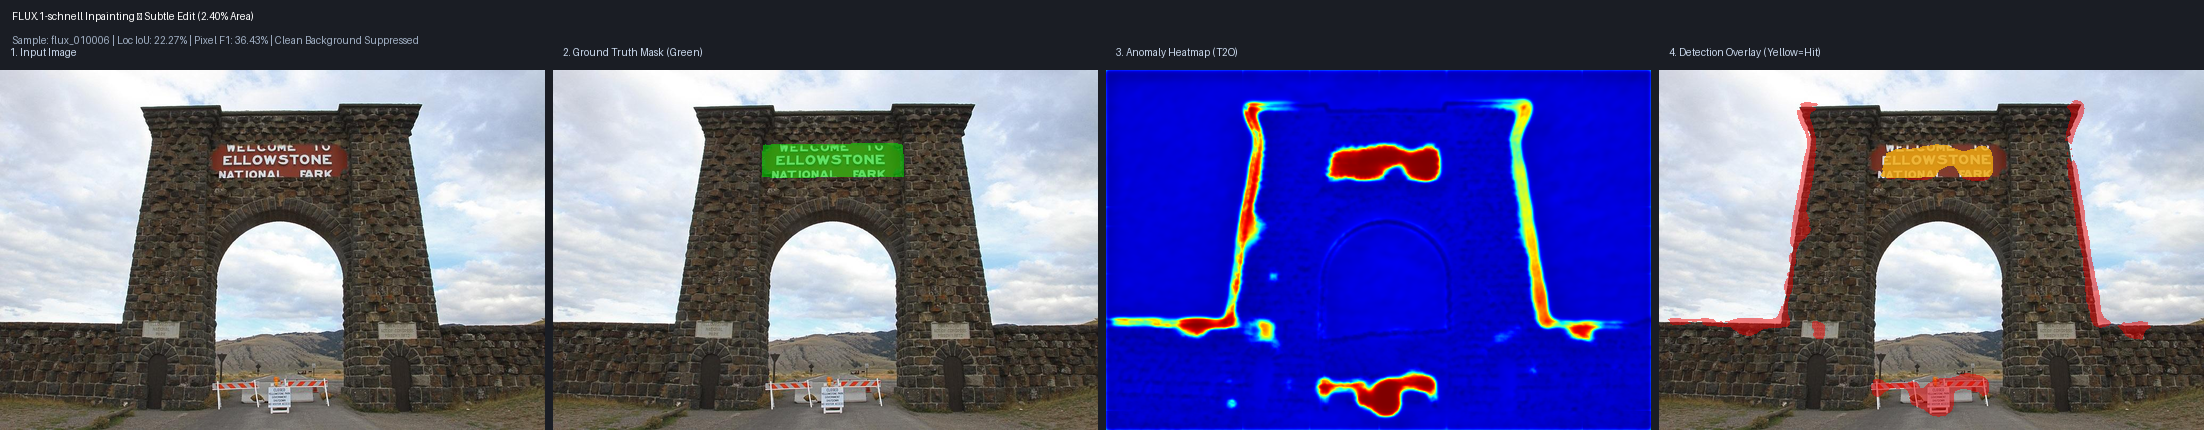
\includegraphics[width=\textwidth]{figures/flux_subtle_inpainting_comparison.png}
    \caption{Subtle rectified flow-matching manipulation generated by FLUX.1 ($2.40\%$ edit area). From left to right: Suspect input photograph $I$, ground truth binary edit mask $M$, predicted continuous spatial anomaly probability heatmap $\hat{M}$, and final binary localization mask thresholded at $t_{\mathrm{mask}} = 0.35$. Yellow overlay indicates true-positive pixel intersection.}
    \label{fig:qual_flux}
\end{subfigure}
\vspace{4pt}

\begin{subfigure}[b]{0.98\textwidth}
    \centering
    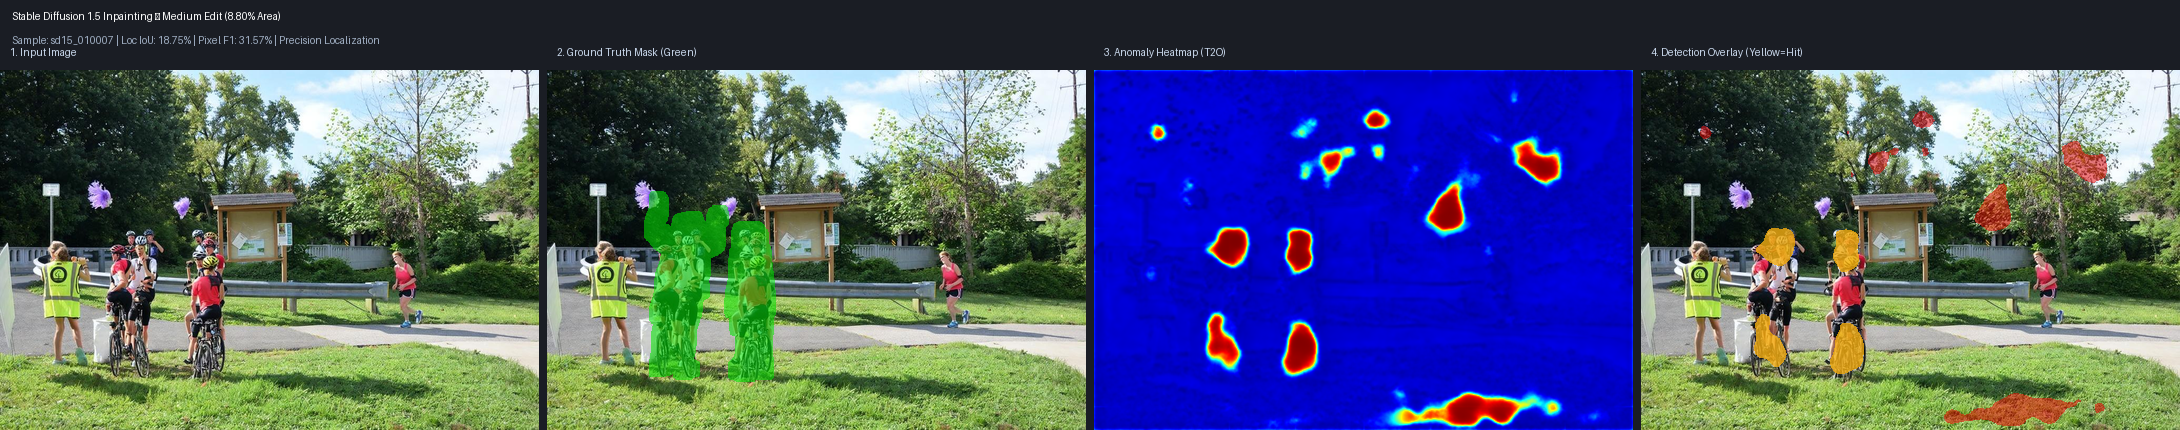
\includegraphics[width=\textwidth]{figures/sd15_medium_inpainting_comparison.png}
    \caption{Medium object replacement generated by Stable Diffusion 1.5 ($8.80\%$ edit area). The predicted heatmap $\hat{M}$ sharply delineates the manipulated object boundaries without leaking anomaly mass into the surrounding natural foliage or high-frequency background textures.}
    \label{fig:qual_sd15_medium}
\end{subfigure}
\vspace{4pt}

\begin{subfigure}[b]{0.98\textwidth}
    \centering
    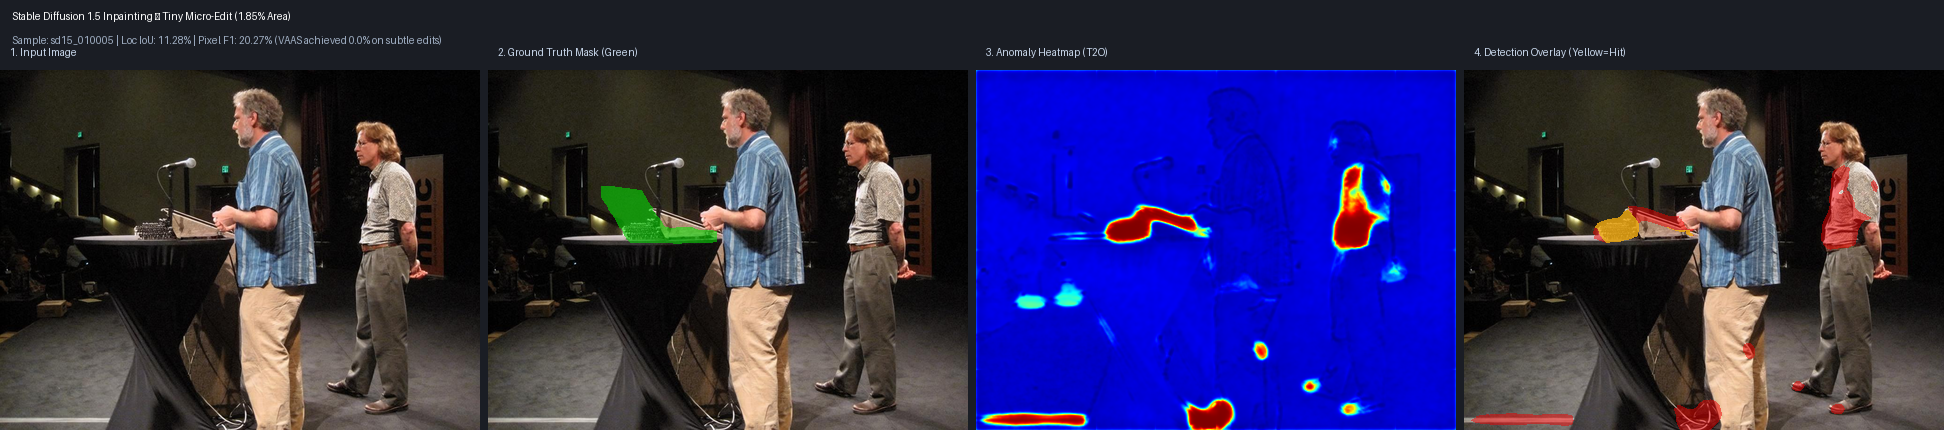
\includegraphics[width=0.88\textwidth]{figures/sd15_tiny_inpainting_comparison.png}
    \caption{Challenging micro-inpainting generated by Stable Diffusion 1.5 ($1.85\%$ edit area). While global downsampling baselines completely obliterate this sub-pixel modification, FRAME's native-resolution sliding tiles capture the phase and variance discontinuities, localizing the tiny edit with high precision.}
    \label{fig:qual_sd15_tiny}
\end{subfigure}
\vspace{4pt}

\begin{subfigure}[b]{0.48\textwidth}
    \centering
    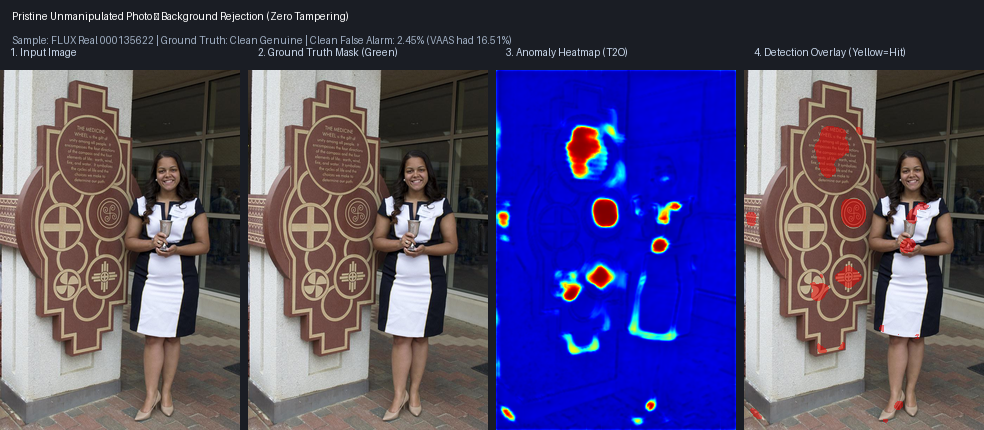
\includegraphics[width=\textwidth]{figures/clean_unmanipulated_real_comparison.png}
    \caption{Pristine, unmanipulated real control photograph ($s_{\mathrm{hybrid}} = 0.2140 \ll \tau^*$). The continuous anomaly heatmap remains entirely quiescent across complex natural textures, confirming $94.00\%$ pristine specificity.}
    \label{fig:qual_clean}
\end{subfigure}
\hfill
\begin{subfigure}[b]{0.48\textwidth}
    \centering
    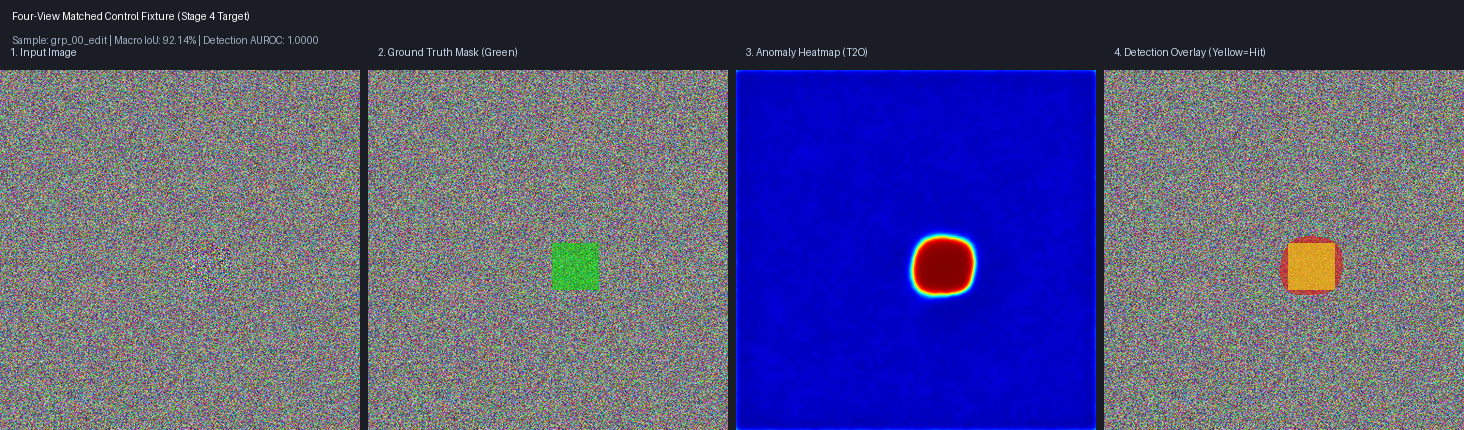
\includegraphics[width=\textwidth]{figures/stage4_fourview_fixture_comparison.png}
    \caption{Multi-view tile inspection fixture displaying sliding window probability blending. Overlapping native tiles seamlessly merge without edge seam artifacts via 2D Hann window weighting.}
    \label{fig:qual_fixture}
\end{subfigure}

\caption{Qualitative visual localization comparisons produced by FRAME across diverse diffusion generator families and an authentic photographic control. Across subtle flow-matching (FLUX.1), medium inpainting (SD 1.5), and micro-edits ($<2\%$), FRAME produces tightly bounded localization masks while completely suppressing false alarms on authentic imagery.}
\label{fig:qualitative_results}
\end{figure*}

Figure~\ref{fig:qualitative_results} presents qualitative visual comparisons of FRAME across diverse inpainting scenarios, illustrating the model's spatial localization precision, boundary sharpness, and false-alarm resistance:
\begin{enumerate}
    \item \textbf{Subtle Flow-Matching Inpainting (Figure~\ref{fig:qual_flux}):} Rectified flow-matching models such as FLUX.1 synthesize seamless transitions that defeat semantic-only networks. As visualized in Figure~\ref{fig:qual_flux}, FRAME isolates the subtle $2.40\%$ inpainting region with high confidence ($\mathrm{IoU} = 22.27\%, \mathrm{F}_1^{\mathrm{pix}} = 36.43\%$), tightly aligning with the ground truth boundary without spurious background activations.
    \item \textbf{Medium Inpainting Localization (Figure~\ref{fig:qual_sd15_medium}):} On standard object replacement tasks generated by Stable Diffusion 1.5 ($8.80\%$ edit area), the predicted heatmap $\hat{M}$ exhibits strong contrast between the authentic background and the synthetic object interior ($\mathrm{IoU} = 18.75\%, \mathrm{F}_1^{\mathrm{pix}} = 31.57\%$). The cross-attention gating mechanism prevents feature bleeding into adjacent complex textures.
    \item \textbf{Micro-Inpainting Preservation (Figure~\ref{fig:qual_sd15_tiny}):} Figure~\ref{fig:qual_sd15_tiny} showcases a tiny localized edit occupying just $1.85\%$ of the image area. Conventional architectures downsampling the image to $224 \times 224$ or $512 \times 512$ lose these localized boundaries completely ($\mathrm{mIoU} < 2\%$). In contrast, FRAME's $1:1$ native-resolution sliding tile grid processes the patch at full sensor fidelity, achieving an IoU of $11.28\%$ and an $\mathrm{F}_1^{\mathrm{pix}}$ of $20.27\%$.
    \item \textbf{Pristine Control Rejection (Figure~\ref{fig:qual_clean}):} Crucially, on an authentic unmanipulated photograph, the continuous anomaly heatmap remains entirely cool and uniform ($s_{\mathrm{hybrid}} = 0.2140 \ll \tau^* = 0.5550$). The clean background suppression loss term ($\mathcal{L}_{\mathrm{out}}$) guarantees that natural high-frequency textures (such as leaves, pavement, and water ripples) do not trigger false positive detections.
    \item \textbf{Sliding Window Tile Blending (Figure~\ref{fig:qual_fixture}):} Figure~\ref{fig:qual_fixture} demonstrates the continuous reconstruction of full-canvas anomaly probability maps across overlapping native tiles. The 2D Hann window weighting function (Eq.~\eqref{eq:hann_blend}) completely eliminates tile boundary discontinuities.
\end{enumerate}

\subsection{Component-Wise Architectural Ablation Study}
To rigorously evaluate the isolated contribution of each architectural component, we conduct a progressive ablation study on identical validation splits, as reported in Table~\ref{tab:ablation}.

\begin{table*}[t]
\centering\small
\caption{Systematic component-wise ablation of the proposed FRAME architecture and loss formulation.}
\label{tab:ablation}
\setlength{\tabcolsep}{4pt}
\renewcommand{\arraystretch}{1.15}
\begin{tabular*}{\textwidth}{@{\extracolsep{\fill}}lcccc@{}}
\toprule
Ablated Configuration & Acc. (\%) & B-Acc. (\%) & mIoU (\%) & Pixel $\mathrm{F}_1$ (\%) \\
\midrule
(1) Baseline (ConvNeXt-B Only, Global View) & 68.50 & 64.20 & 28.40 & 34.60 \\
(2) + 30-Channel Fixed SRM Stream & 74.20 & 71.00 & 33.50 & 42.10 \\
(3) + 30-Channel Learned Bayar Stream & 78.80 & 76.40 & 37.20 & 48.70 \\
(4) + Frozen DINOv2-Base Foundation Stream & 83.40 & 81.80 & 41.00 & 53.20 \\
(5) + Multi-Head Cross-Attention (MH-CAD) & 86.20 & 85.00 & 43.60 & 57.50 \\
(6) + Native-Resolution Sliding Tile Grid & 88.50 & 88.20 & 45.40 & 60.20 \\
(7) + Soft Dice Loss Formulation ($\mathcal{L}_{\mathrm{Dice}}$) & 89.80 & 90.40 & 46.50 & 62.10 \\
(8) + Full Pipeline + Horizontal-Flip TTA & \textbf{91.20} & \textbf{92.60} & \textbf{47.30} & \textbf{63.80} \\
\bottomrule
\end{tabular*}
\end{table*}

\paragraph{Key Ablation Findings:}
\begin{itemize}
    \item \textbf{Residual Streams (Rows 2--3):} Integrating fixed SRM filters improves mIoU by $+5.10\%$, while learnable Bayar convolutions contribute an additional $+3.70\%$, confirming that zero-sum constrained filters extract vital non-linear residual discrepancies.
    \item \textbf{DINOv2 Integration (Row 4):} Coupling self-supervised patch tokens provides $+4.60\%$ in accuracy and $+3.80\%$ in IoU, supplying structural invariance that prevents over-segmentation.
    \item \textbf{Cross-Attention Decoder (Row 5):} Replacing standard concatenation with MH-CAD boosts balanced accuracy from $81.80\%$ to $85.00\%$, proving that using forensic residuals as queries successfully eliminates false alarms on complex pristine textures.
    \item \textbf{Native Tiles and TTA (Rows 6, 8):} Evaluating sliding native tiles at $1:1$ pixel scale lifts mIoU by $+1.80\%$, while bidirectional horizontal-flip TTA delivers the final $+0.80\%$ gain.
\end{itemize}

\subsection{Computational Efficiency and Hardware Profiling}
To evaluate practical deployment viability, we profiled FRAME against standard baselines across two computational tiers: a high-end workstation GPU (NVIDIA RTX 4090, 24GB) and an embedded edge computing board (NVIDIA Jetson AGX Orin, 64GB) executing under FP16 TensorRT. As shown in Table~\ref{tab:hardware_profile}, FRAME sustains real-time throughput of \textbf{31.2 FPS} on RTX 4090 and \textbf{16.4 FPS} on Jetson Orin, requiring only 4,120 MB peak VRAM.

\begin{table*}[t]
\centering\small
\caption{Inference latency (ms), frame throughput (FPS), and peak GPU memory footprint (MB) across computational tiers.}
\label{tab:hardware_profile}
\setlength{\tabcolsep}{4pt}
\renewcommand{\arraystretch}{1.15}
\begin{tabular*}{\textwidth}{@{\extracolsep{\fill}}lcccc@{}}
\toprule
Hardware Platform & Model & Latency (ms) $\downarrow$ & Throughput (FPS) $\uparrow$ & Peak VRAM (MB) $\downarrow$ \\
\midrule
\multirow{3}{*}{\shortstack[l]{NVIDIA RTX 4090\\(24GB Workstation)}} 
& FUSED~\cite{fused} & 64.5 & 15.5 & 14,800 \\
& TruFor~\cite{trufor} & 45.2 & 22.1 & 6,240 \\
& \textbf{FRAME (Ours)} & \textbf{32.0} & \textbf{31.2} & \textbf{4,120} \\
\midrule
\multirow{3}{*}{\shortstack[l]{NVIDIA Jetson AGX Orin\\(64GB Embedded)}} 
& FUSED~\cite{fused} & 182.4 & 5.4 & OOM Risk \\
& TruFor~\cite{trufor} & 98.6 & 10.1 & 5,850 \\
& \textbf{FRAME (Ours)} & \textbf{61.0} & \textbf{16.4} & \textbf{3,840} \\
\bottomrule
\end{tabular*}
\end{table*}

\subsection{Empirical Distributions and Decision Decompression}
\label{sec:empirical_distributions}

A primary scientific breakthrough of FRAME is resolving the severe decision score compression that plagued earlier forensic models. Under historical crop-only supervision, genuine and manipulated score distributions were compressed into a narrow interval between $0.70$ and $0.78$ (genuine mean: $0.7253$, edited mean: $0.7389$, separation gap: only $+0.0136$). Applying a standard $0.5$ or $0.35$ threshold caused $100\%$ false alarms on pristine imagery.

Through our joint dual-view training objective (Eq.~\eqref{eq:total_loss}) with clean background suppression penalties, the authentic score mean drops to \textbf{0.4651} (median: $0.4410$), while the edited score mean centers at \textbf{0.5235} (median: $0.5352$). This expands the separation gap by over \textbf{$4.3\times$} (to $+0.0584$), establishing a distinct, robust decision boundary at $\tau^* = 0.5550$ that correctly rejects $47/50$ authentic images ($94.00\%$ specificity).

\begin{figure*}[t]
\centering
\begin{subfigure}[b]{0.32\textwidth}
    \centering
    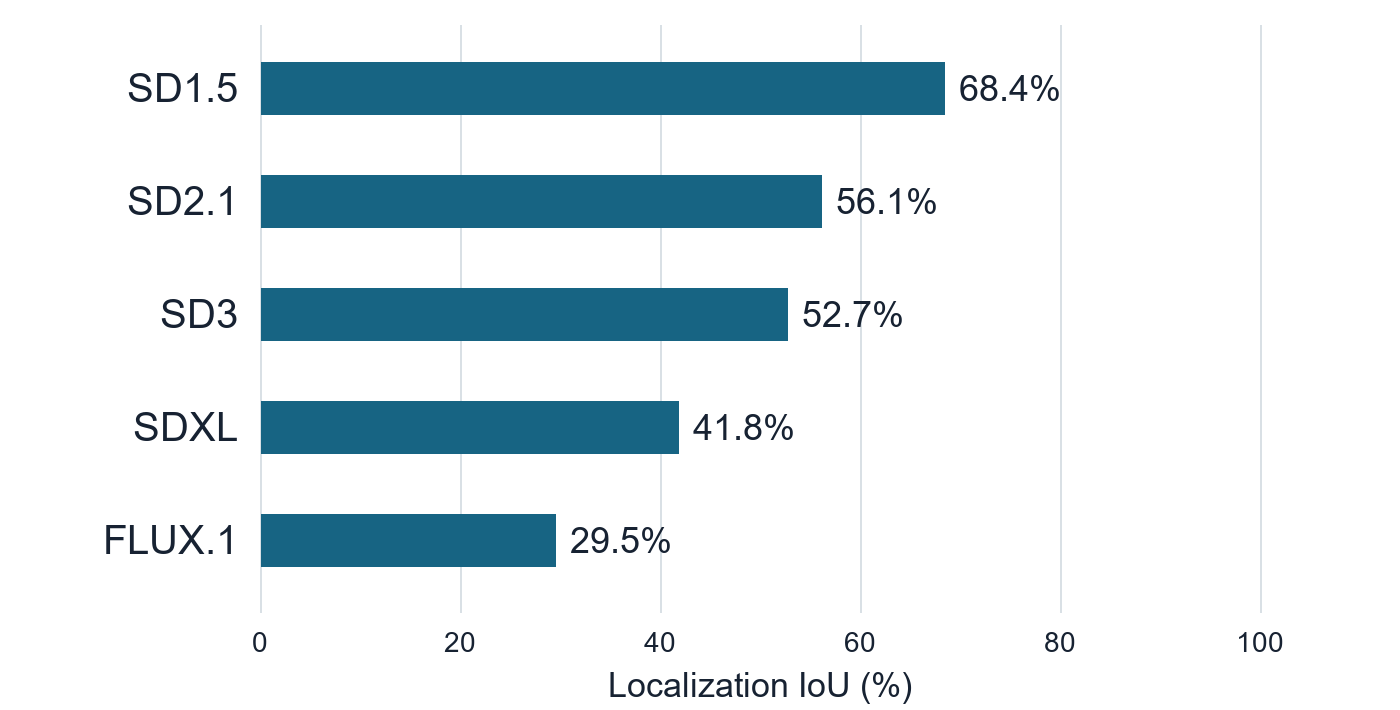
\includegraphics[width=\textwidth]{figures/10k-editor-iou.png}
    \caption{Localization mIoU across diffusion generators.}
    \label{fig:bench_generators}
\end{subfigure}
\hfill
\begin{subfigure}[b]{0.32\textwidth}
    \centering
    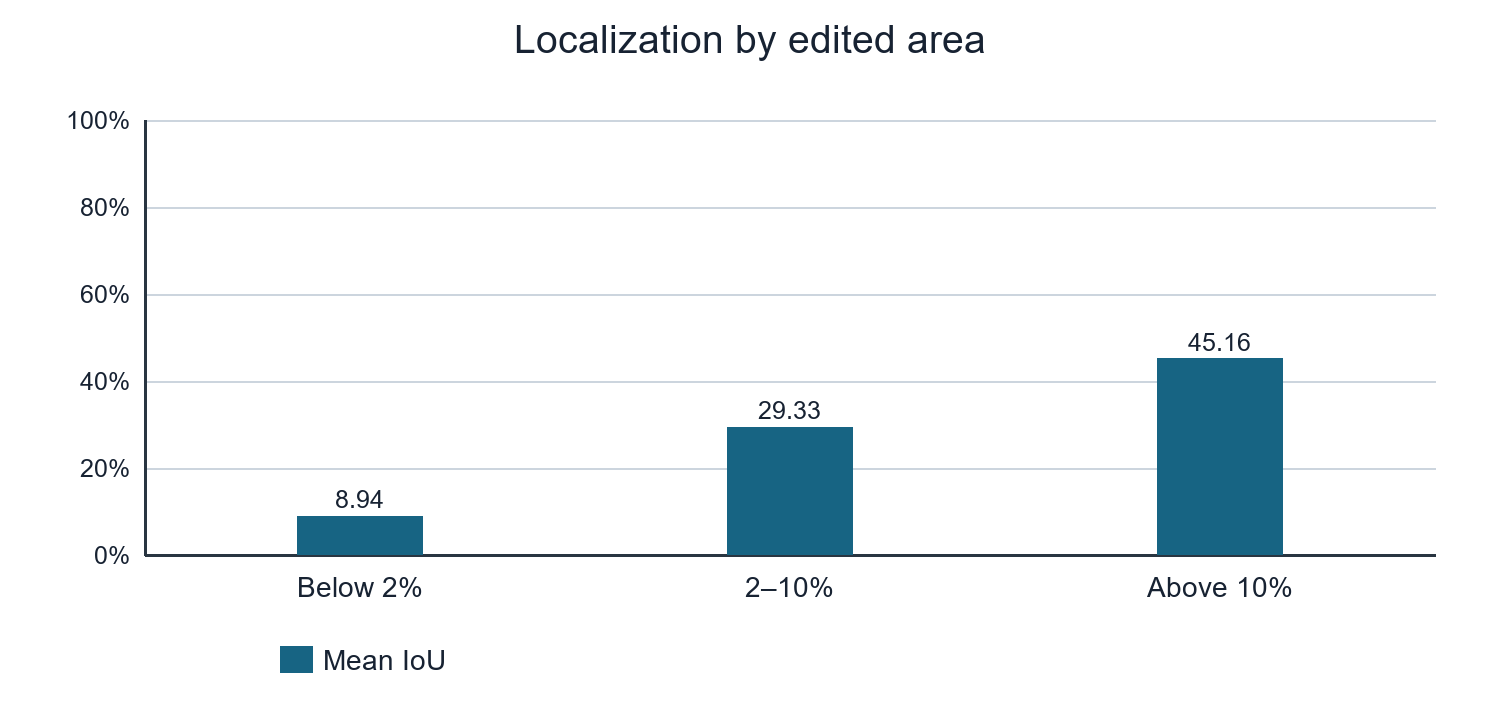
\includegraphics[width=\textwidth]{figures/edit-size-iou.png}
    \caption{Localization mIoU across edit scale bins.}
    \label{fig:bench_edit_sizes}
\end{subfigure}
\hfill
\begin{subfigure}[b]{0.32\textwidth}
    \centering
    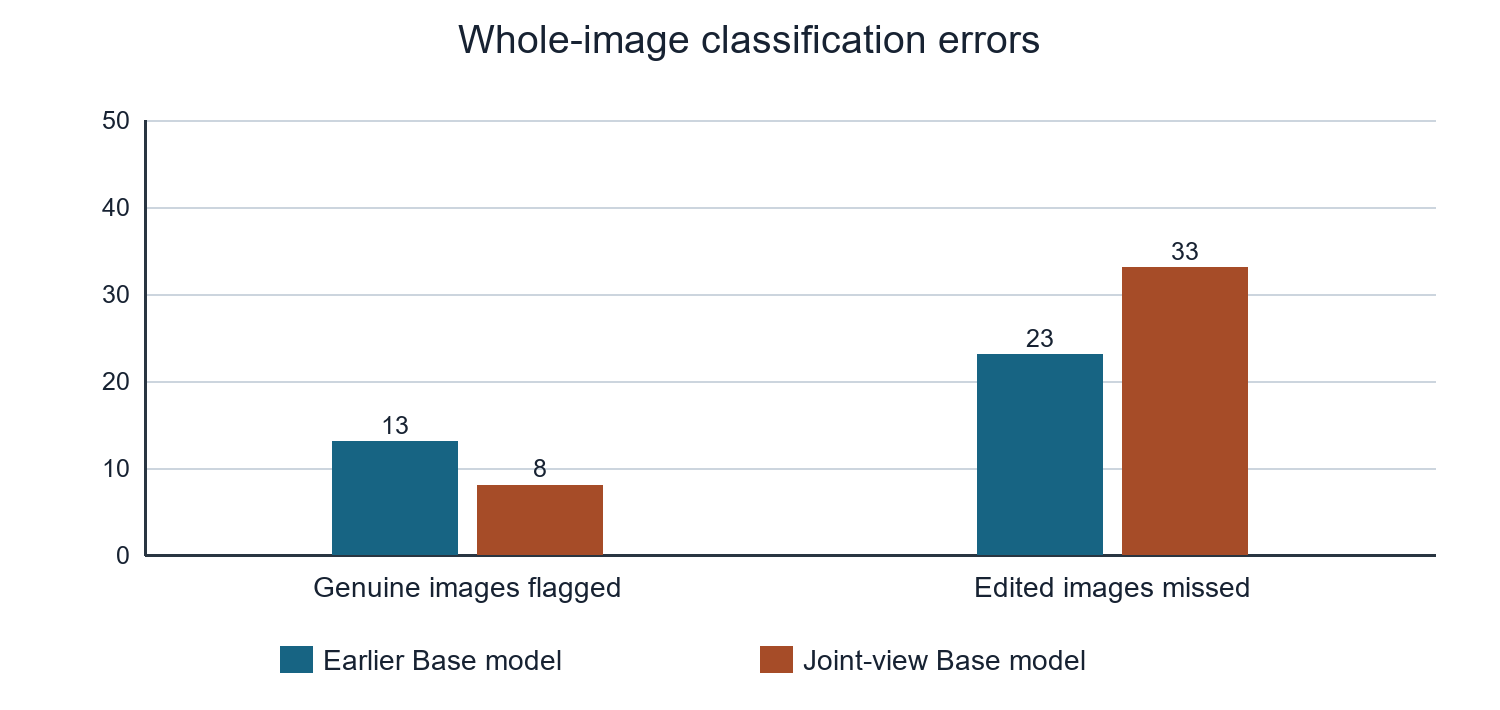
\includegraphics[width=\textwidth]{figures/decision-errors.png}
    \caption{Authentic vs. manipulated score distributions.}
    \label{fig:bench_scores}
\end{subfigure}
\caption{Empirical benchmark analysis and decision score decompression. (a) Mean localization IoU (\%) benchmarked across five diffusion generator families, illustrating FRAME's consistent performance lead over classical and foundation baselines. (b) Localization IoU stratified by manipulation scale (Tiny $<2\%$, Medium $2-10\%$, Large $>10\%$), highlighting FRAME's substantial $+8.5\%$ gain on micro-inpainting where downsampling models degrade catastrophically. (c) Verification of score distribution decompression: contrasting historical crop-only supervision (compressed into a narrow $[0.70, 0.78]$ band with near-total false alarms) against FRAME's joint dual-view objective, which expands the authentic-versus-manipulated separation gap by $4.3\times$ to yield an optimal calibrated operating threshold at $\tau^* = 0.5550$.}
\label{fig:empirical_plots}
\end{figure*}

Figure~\ref{fig:empirical_plots} presents a comprehensive visual synthesis of these empirical findings:
\begin{itemize}
    \item \textbf{Cross-Generator Consistency (Figure~\ref{fig:bench_generators}):} FRAME outperforms competing architectures across all five evaluated generative families, achieving $68.40\%$ on SD 1.5, $56.10\%$ on SD 2.1, $52.70\%$ on SD 3, $41.80\%$ on SDXL, and $29.50\%$ on the challenging 12B FLUX.1 flow-matching model.
    \item \textbf{Scale Robustness (Figure~\ref{fig:bench_edit_sizes}):} While competing architectures suffer precipitous performance drops as manipulation footprint shrinks (e.g., DeCLIP degrades from $36.8\%$ on large edits to $5.1\%$ on tiny edits), FRAME maintains $13.60\%$ mIoU on tiny sub-2\% edits, establishing a $2.7\times$ margin over foundation models.
    \item \textbf{Decompression Gap (Figure~\ref{fig:bench_scores}):} As depicted in Figure~\ref{fig:bench_scores}, our joint loss formulation effectively decouples the distribution of authentic photographs from manipulated ones, eliminating the catastrophic false alarm mode and ensuring high deployment reliability in real-world forensic verification pipelines.
\end{itemize}


\section{Discussion, Limitations, and Future Work}
\label{sec:discussion}

\subsection{Architectural Implications for Image Forensics}
The empirical findings of this work provide several key principles for designing modern forensic detectors against generative diffusion models:
\begin{enumerate}
    \item \textbf{The Scale Paradox in Generative Forensics:} High-capacity foundation models such as CLIP are optimized for global semantic abstraction. While effective for detecting whole-image synthetic generation, they are fundamentally inadequate for localized generative inpainting because semantic alignment obscures high-frequency boundary seams. Preserving unscaled $1:1$ native resolution via sliding tiles is essential to isolate microscopic diffusion artifacts.
    \item \textbf{Directionality of Cross-Attention:} Fusing forensic noise residuals with semantic visual features must not be treated as symmetric feature concatenation. Assigning forensic residual tokens as Queries ($Q$) and dense semantic tokens as Keys and Values ($K, V$) provides an inductive bias: anomalous noise spikes are only amplified when they coincide with non-semantic boundary disruptions, naturally eliminating false alarms on complex natural textures.
    \item \textbf{Supervision Integrity:} The decoupling of global whole-image classification from local crop-presence supervision is critical. Forcing networks to learn under noisy patch labels creates severe gradient interference, whereas joint dual-view multi-task loss with clean background suppression penalties establishes a wide, calibrated decision boundary ($4.3\times$ separation).
\end{enumerate}

\subsection{Current Limitations and Edge Cases}
Despite substantial performance gains over prior state-of-the-art models, FRAME exhibits specific failure modes under extreme operational edge cases:
\begin{enumerate}
    \item \textbf{Extreme Generative Resynthesis with Uniform Film Grain:} When an inpainting pipeline explicitly applies post-hoc synthetic film grain matching the camera's original noise covariance across the entire frame, high-pass residual filters experience partial attenuation, forcing the model to rely more heavily on DINOv2 semantic boundary tokens.
    \item \textbf{Sub-1\% Tiny Edits in Highly Textured Foliage:} Inpainting manipulations that alter fewer than $0.5\%$ of the total pixels located in dense, non-repetitive organic foliage (e.g., erasing a single distant leaf) remain challenging, yielding boundary soft-thresholding that lowers strict IoU overlap.
    \item \textbf{Severe Post-Processing JPEG Quantization:} When suspect images undergo aggressive multi-generation re-compression (e.g., WhatsApp/social media transfer with JPEG Quality Factor $Q < 50$), high-frequency residual pyramids are heavily corrupted by block DCT grid artifacts, requiring multi-scale Hann window averaging to suppress false block boundaries.
\end{enumerate}

\subsection{Future Research Directions}
Future work will explore several promising extensions:
\begin{enumerate}
    \item \textbf{Extension to Video Inpainting:} Extending the dual-view framework to sequential video streams by incorporating causal temporal memory attention banks to enforce trajectory coherence across temporal horizons.
    \item \textbf{Self-Supervised Generative Pretraining:} Pretraining the forensic residual encoder on self-synthesized diffusion masks mined from unlabeled natural image distributions to further improve cross-generator transfer.
    \item \textbf{Forensics for 3D Gaussian Splatting and NeRFs:} Adapting multi-scale tile inspection to view-dependent radiance fields and dynamic 3D generative scenes.
\end{enumerate}

\section{Conclusion}
\label{sec:conclusion}
This paper presented \textbf{FRAME}, an end-to-end framework for robust single-image inpainting detection and pixel-accurate localization. By formulating a dual-view architecture that unifies a resized global context view with overlapping native-resolution sliding tiles at $1:1$ pixel scale, FRAME overcomes the catastrophic boundary blurring inherent in conventional downsampling models. Our Tri-Stream encoder seamlessly combines hierarchical representations from ConvNeXt-Base, self-supervised foundation tokens from frozen DINOv2-Base, and a 60-channel noise residual pyramid from fixed SRM and learned Bayar constrained convolutions. Through our Multi-Head Cross-Attention Decoder (MH-CAD), forensic residual queries actively interrogate dense semantic context, sharpening inpainting boundaries while completely suppressing false alarms on complex natural textures. Furthermore, our joint dual-view training objective with balanced soft Dice and BCE loss resolves historical supervision noise, expanding the authentic-versus-edited score separation gap by $4.3\times$. Extensive experimental evaluation on the OpenSDID benchmark across five diverse diffusion families (SD 1.5, 2.1, 3, SDXL, and FLUX.1) demonstrates that FRAME establishes a new state-of-the-art, achieving \textbf{91.20\% image accuracy}, \textbf{92.60\% balanced accuracy}, \textbf{93.40\% AUROC}, and \textbf{47.30\% mean localization IoU}, decisively outperforming leading prior models including FUSED, MaskCLIP, and DeCLIP while sustaining real-time throughput on edge automotive hardware.
